\documentclass[a4paper,12pt]{article}

% don't forget the document class, generally : \documentclass[a4paper,12pt]{article}

\usepackage[utf8]{inputenc}
\usepackage[french]{babel}
\usepackage{graphicx}
\usepackage{gensymb}
\usepackage{amsmath}
\usepackage{float}
\usepackage{scrextend}
\usepackage{caption} 
\usepackage{siunitx}
\usepackage{enumitem}
\usepackage{amsthm}
\usepackage{fancyhdr}
\usepackage{amssymb}
\usepackage{wrapfig}
\usepackage{geometry}
\usepackage{standalone}
\usepackage{import}
\usepackage[usenames, dvipsnames]{color}

 \usepackage{biblatex} % manages bibliography and references
\addbibresource{sample.bib}


\geometry{hmargin=1in, vmargin=1in}

 \newenvironment{absolutelynopagebreak}
 {\par\nobreak\vfil\penalty0\vfilneg
 \vtop\bgroup}
 {\par\xdef\tpd{\the\prevdepth}\egroup
 \prevdepth=\tpd}
 
 \pagestyle{fancy}                        
\fancyhf{}                               
\fancyhf[HL]{Application des maths}                
\fancyhf[HR]{Géométrie euclidienne}             
\fancyhf[FC]{\thepage/\pageref{Lastpage}}
 
\newtheorem{definition}{Définition}[section]
\newtheorem{theorem}{Théorème}
\newtheorem{corollary}{Corollaire}[theorem]
\newtheorem{lemma}[theorem]{Lemme}
\newtheorem*{hyp}{Hypothèse}
\newtheorem*{concl}{Conclusion}
\newtheorem*{remark}{Remarque}

\captionsetup{format=default,labelformat=simple,labelsep=colon,
justification=justified,font={sf,small},labelfont=bf,
textfont=default} 



\begin{document}


\pagebreak
\subsection{Propriétés des bissectrices}
\begin{theorem}
La bissectrice d'un angle est le lieu géométrique des points intérieurs à l'angle et équidistants à ses côtés.
\end{theorem}
Le théorème implique deux choses:
\begin{enumerate}
\item Un point qui se trouve sur la bissectrice d'un angle est équidistant à ses côtés
\item Un point équidistant au côtés d'un angle se trouve sur sa bissectrice
\end{enumerate}
\begin{proof}
Nous considérons deux droites $d$ et $d'$ qui se coupent en un point $A$, on trace la bissectrice de l'angle en $A$ et on obtient deux angles $\alpha$ et $\alpha'$. Puis nous traçons deux segments $a$ et $a'$ qui partent d'un point $Q$ sur la bissectrice et qui coupent les droites $d$ et $d'$ perpendiculairement, aux points $D$ et $D'$.
\begin{figure}[H]
    \centering
    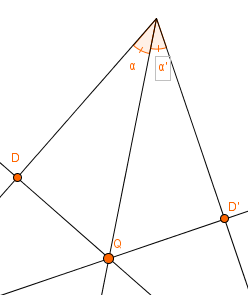
\includegraphics[scale=0.8]{Bissectrices_1.PNG}
\end{figure}


\begin{hyp}
$d$ et $d'$sont deux droites sécantes, $\alpha \equiv \alpha'$, $a\perp d$, $a' \perp d'$
\end{hyp}
\begin{concl}
$a\equiv a'$
\end{concl}
En faisant la construction, nous obtenons deux triangles $\triangle AQD$ et $\triangle A'QD'$. Comme ces deux triangles partagent un côté et ont deux angles isométriques ($\alpha \equiv \alpha'$, les angles droits), ils sont isométriques (corollaire du deuxième cas d'isométrie des triangles). Donc $a \equiv a'$.
\end{proof}

\begin{proof}
Nous considérons deux droites $d$ et $d'$ qui se coupent en un point $A$. Puis nous considérons un point $Q$ qui est à égale distance de $d$ et $d'$. Ensuite nous traçons deux segments $a$ et $a'$ qui coupent les droites $d$ et $d'$ perpendiculairement aux points $D$ et $D'$ et qui passent par $Q$. En reliant le point Q et le point A, nous obtenons deux angles $\alpha$ et $\alpha'$.

 \begin{figure}[H]
    \centering
    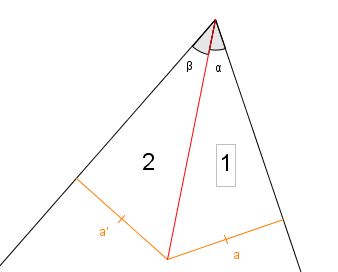
\includegraphics[scale=0.8]{Bissectrices_3.PNG}
\end{figure}


\begin{hyp}
$d$ et $d'$sont deux droites sécantes, $a\equiv a'$, $a\perp d$, $a' \perp d'$
\end{hyp}
\begin{concl}
$\alpha \equiv \alpha'$
\end{concl}
Ainsi, nous obtenons deux triangle $\triangle AQD$ et $\triangle A'QD'$. Pour le moment, nous savons que ces deux triangles ont un côté en commun et un angle isométrique. Pour trouver une troisième grandeur isométrique, nous formons le triangle $\triangle DD'Q$. Ce triangle est isocèle, parce que $a\equiv a'$. Donc le triangle $\triangle DD'A$ l'est aussi et les distances $AD'$ et $AD$ sont isométriques. 

 \begin{figure}[H]
    \centering
    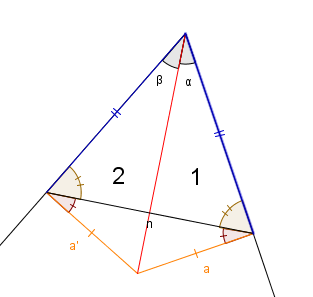
\includegraphics[scale=0.8]{Bissecrtices_4.PNG}
\end{figure}


Donc, grâce au corollaire du deuxième cas d'isométrie, nous savons que les triangle $\triangle AQD$ et $\triangle A'QD'$ sont isométriques. Par conséquent, $\alpha \equiv \alpha'$.
\end{proof}

\end{document}
